\section{Testing}

Consider the function \texttt{bar}, written in a C-like language:
\begin{lstlisting}[style=C]
0: int bar(int a, int b, int c) {
1:      int h = b-2;
2:      if (a < h) {
3:          if (a == h+2)
4:              return c;
5:          else if (a < b-3)
6:              h = a;
7:      }
8:      return h; 
9: } 
\end{lstlisting}
\begin{enumerate}
    \item Derive the Control Flow Graph of the given function.
    \item Derive the set of live variables at the exit of each block.
        Are there dead variables after definition at block 0?
    \item Use symbolic execution to explore all paths in the function. 
\end{enumerate}

\paragraph*{Solution}
\begin{enumerate}
    \item The Control Flow Graph of the function is derived from the code and is the following: 
        \begin{figure}[H]
            \centering
            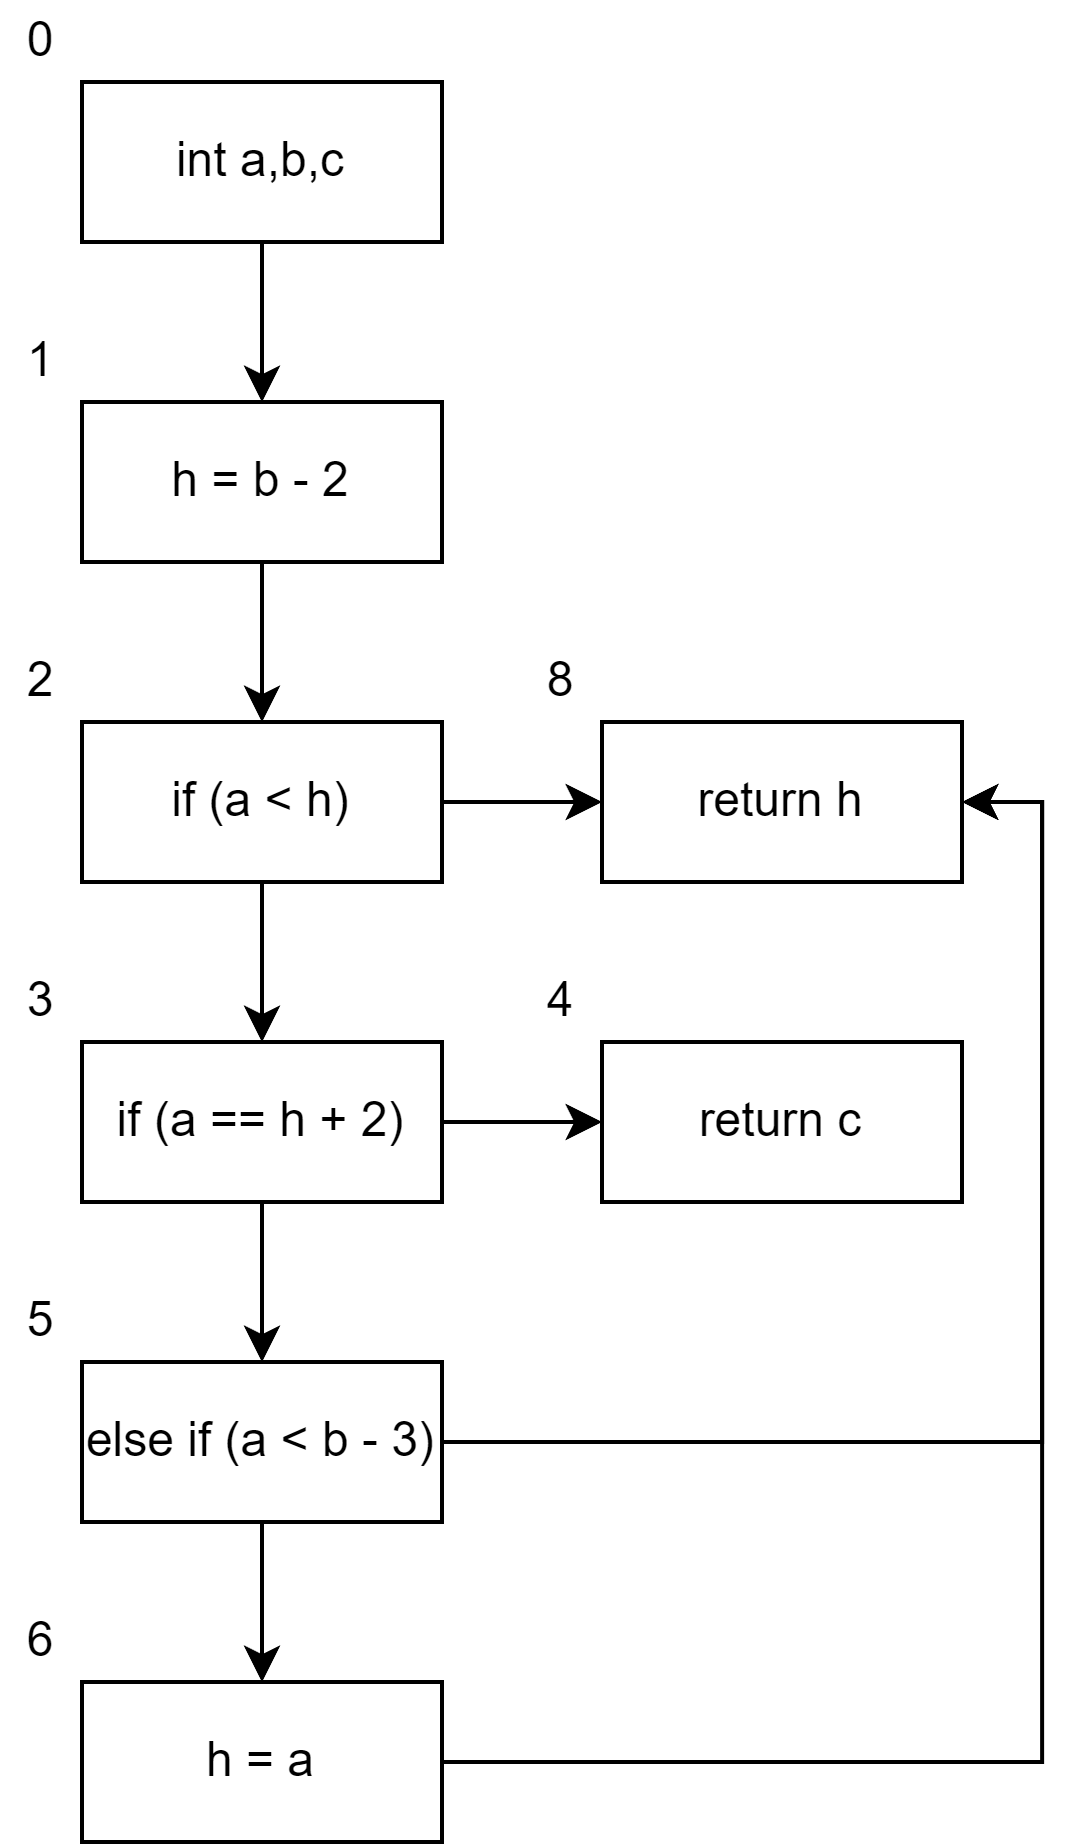
\includegraphics[width=0.4\linewidth]{images/cfg.png}
        \end{figure}
    \item The definition of live variable is the following: "Given a CFG, a variable v is live at the exit of a block b if there is some path (on the CFG) from block b to a use of v that does not redefine v". 
        By exploiting this definition we have to check all variables that are live in the node by checking if there is a path from the node that uses the variable without redefining it. 
        With this analysis we find the following: 
        \begin{itemize}
            \item $\text{LV}(0) = \{a,b,c\}$
            \item $\text{LV}(1) = \{a,b,c,h\}$
            \item $\text{LV}(2) = \{a,b,c,h\}$
            \item $\text{LV}(3) = \{a,b,c,h\}$ 
            \item $\text{LV}(4) = \{ \}$ 
            \item $\text{LV}(5) = \{a,h\}$ 
            \item $\text{LV}(6) = \{h\}$ 
            \item $\text{LV}(8) = \{ \}$
        \end{itemize}
    \item The possible paths are: 
        \begin{itemize}
            \item $\left\langle 0,1,2,3,5,6,8 \right\rangle$: that is feasible with the condition $A < B-3$. 
            \item $\left\langle 0,1,2,3,5,8 \right\rangle$: that is feasible with the condition $A=B-3 $. 
            \item $\left\langle 0,1,2,8 \right\rangle$: that is feasible with the condition $A \geq B-2$. 
        \end{itemize}
\end{enumerate}